%Exemplo de capitulo

\chapter{Redes Neurais Convolucionais}
\setcounter{figure}{100}

Rede neural artificial (\sigla{ANN}{\emph{Artificial Neural Network},
rede neural artificial}) é um modelo computacional inspirado na forma com
que o cérebro resolve problemas \cite{gilbert2000build}. Este modelo possui
unidades, denominadas neurônios, que possuem um valor que é calculado como uma
função do valor de outros neurônios.

\begin{figure}[!htb]
	\centering
	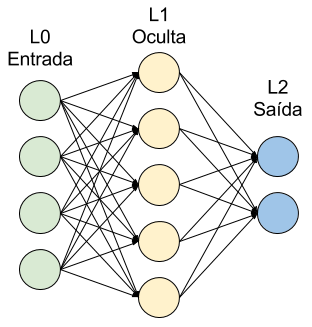
\includegraphics{ex_fcnn.png}
	\caption{Exemplo de rede neural totalmente conectada}
	\label{fig:ex_fcnn}
	(próprio autor).
\end{figure}

Alguns neurônios especiais, denominados “entradas” possuem um valor obtido de
fora do sistema. Estes são especiais porque são os únicos cujos valores não são
calculados. O valor de alguns dos neurônios de uma rede neural artificial podem
afetar sistemas externos à ela. Por isso são designados “saídas”. Neurônios que
não são de entrada ou de saída são chamados “ocultos”. A figura
\ref{fig:ex_fcnn} ilustra uma rede neural simples com os três tipos de
neurônios.

\section{Redes Neurais Não-Convolucionais}
As redes neurais artificiais são tipicamente organizadas em “camadas”, e a
escolha dos tipos de neurônio, juntamente com a forma com que os neurônios são
conectados, é denominada “topologia”. As redes são classificadas como
feedforward quando as conexões não formam ciclos ou recurrent quando formam. Se
uma camada está conectada a todos os neurônios da camada anterior diz-se que a
camada é totalmente conectada.
A definição da função de transferência do neurônio é uma parte importante da
topologia das redes neurais. Um tipo muito comum de neurônio é definido por:

\begin{equation} \label{eq:non-conv-layer}
	v=A \left( \left( \sum_n w_n i_n \right) + b \right)
\end{equation}

Onde $v$ é o valor do neurônio, $i_n$ é n-ésima entrada do neurônio,
$w$ é um vetor de escalares denominado peso, e $b$ é um escalar arbitrário,
denominado bias. A é uma
função denominada função de ativação do neurônio. Essa função pode ser usada
para tornar o neurônio não-linear, como no caso da tangente hiperbólica. Os
pesos determinam a influência de cada entrada do neurônio.

A descrição de redes neurais com este tipo de neurônio e com topologia
totalmente conectada é especialmente conveniente. As três camadas
da rede neural ilustrada na figura \ref{fig:ex_fcnn} podem ser representadas
por matrizes:

\noindent\begin{minipage}{.333\linewidth}
	\begin{equation} \label{eq:l0}
		L0_{4 \times 1} =
			\begin{pmatrix}
				a_1 \\
				a_2 \\
				a_3 \\
				a_4
			\end{pmatrix}
	\end{equation}
\end{minipage}
\begin{minipage}{.333\linewidth}
	\begin{equation} \label{eq:l1}
		L1_{5 \times 1} =
			\begin{pmatrix}
				b_1 \\
				b_2 \\
				b_3 \\
				b_4 \\
				b_5
			\end{pmatrix}
	\end{equation}
\end{minipage}
\begin{minipage}{.333\linewidth}
	\begin{equation} \label{eq:l2}
		L2_{2 \times 1} =
			\begin{pmatrix}
				c_1 \\
				c_2
			\end{pmatrix}
	\end{equation}
\end{minipage}

Para calcular a primeira camada intermediária é preciso aplicar a equação
(\ref{eq:non-conv-layer}) cinco vezes, uma para cada neurônio. Porém, se
esta camada for totalmente conectada, e todos os neurônios usarem a
mesma função de transferência $A$, e a representação em matrizes estiver
sendo usada, o cálculo de todos os neurônios desta camada pode ser
realizado usando:

\begin{equation}
	L1_{5 \times 1}=A_V \left( W1_{5 \times 4} \times L0_{4 \times 1}
		+ B1_{5 \times 1} \right)
\end{equation}

Onde $A_V$ é uma versão vetorial da função de ativação resultante
da aplicação da função $A$ em cada um dos elementos do vetor.
Os pesos dos cinco neurônios, denominados $w_n$ na equação
\ref{eq:non-conv-layer} são aqui representados por uma única matriz
$W1_{5 \times 4}$, e os bias dos cinco neurônios, $b$, são representados por
uma única matriz $B1_5$. Da mesma forma, a camada de saída
pode ser calculada com:

\begin{equation}
	L2_{2 \times 1}=A_V \left( W2_{2 \times 5} \cdot L1_{5 \times 1}
		+ B2_{2 \times 1} \right)
\end{equation}

As matrizes $W$ e $B$ são os parâmetros que precisam ser aprendidos durante o
treinamento, e são denominados parâmetros treináveis. O número de parâmetros
de uma uma
rede neural é igual ao número de valores contidos em todas as matrizes de pesos
e bias. Quanto maior o número de parâmetros, mais flexibilidade a rede neural
possui, porém mais lento é o treinamento. Se o número de parâmetros for
excessivo a rede neural perde a capacidade de generalizar e ocorre
\emph{overfitting}.

De acordo com \cite{hawkins2004problem}, \emph{overfitting} ocorre quando um
modelo é mais flexível do que precisa ser. Quando um modelo destes é treinado,
especialmente com poucos exemplos, o modelo pode acabar ``memorizando'' os
exemplos, ao invéz de generazar o comportamento geral dos dados, fazendo
com que o resultado da classificação seja bom, mas haja erro excessivo
quando o mesmo modelo é aplicado em dados novos.

Como as dimensões da matriz de pesos são iguais ao número de entradas em uma
direção pelo número de saídas na outra direção, o número de parâmetros nessa
matriz é igual ao produto dos dois. Se uma camada totalmente conectada tem 1000
entradas e 1000 saídas a matriz de pesos vai possuir 1.000.000 de parâmetros
e a matriz de \emph{bias} mais 1.000, resultando em um total de 1.001.000
parâmetros.

\section{Redes Neurais Convolucionais}
Redes neurais convolucionais são um tipo de rede neural que inclui operações
baseadas em uma definição relaxada de convolução. A principal operação
neste tipo de rede neural é a a correlação cruzada (\emph{cross-correlation}).
Para duas funções discretas $f$ e $g$, a correlação cruzada discreta entre
elas é definida por:

\begin{equation}
	def: (f \star g)[n] = \sum_{m=-\infty}^{\infty} f^*[m]g[m+n]
\end{equation}

Onde $f^*$ é o complexo conjugado da função $f$. A figura
\ref{fig:cap2_ex_corr_cruz_1d} ilustra uma operação de correlação cruzada sendo
realizada pelo método visual.

\begin{figure}[!htb]
	\centering
	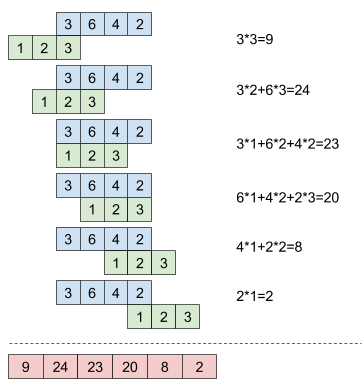
\includegraphics{cap2_ex_corr_cruz_1d.png}
	\caption{Exemplo de correlação cruzada 1D}
	\label{fig:cap2_ex_corr_cruz_1d}
	Na imagem está sendo calculada a correlação cruzada entre $[3,6,4,2]$ e
	$[1,2,3]$. O primeiro set de dados fica fixo enquanto o segundo vai sendo
	deslocado, e em cada vez se calcula a soma do produto, conforme ilustrado.
	O resultando é $[9,24,23,20,8,2]$.
\end{figure}

A correlação cruzada também é definida para dimensões maiores que 1.
Tomando as funções discretas $f[n_1,n_2]$ e $g[n_1,n_2]$ pode-se 
escrever a convolução 2D destas funções como sendo:

\begin{equation}
	def: (f \star\star g)[n_1,n_2] =
		\sum_{m_1=-\infty}^{\infty} \quad
		\sum_{m_2=-\infty}^{\infty}
		f^*[m_1,m_2]g[m_1+n_1,m_2+n_2]
\end{equation}

É possível realizar convoluções para um número arbitrário de dimensões através
da generalização desta equação.

A aplicação do operador de correlação cruzado é próximo ao conceito de filtro
linear, bastante usado em processamento digital de imagens
\cite{gonzalezwoods200708}. Os conceitos não
são idênticos por que filtro digital trata uma das entradas como sendo
``sinal'',
e a outra como sendo o filtro, ou \emph{kernel}, e convoluções e correlações
cruzadas tratam as duas entradas de forma idêntica, e produzem um resultado
diferente nos extremos. Como observa-se na figura
\ref{fig:cap2_ex_corr_cruz_1d}, a saída é um vetor de dimensão 6, e um filtro
digital geraria saída de tamanho 4 (se houvesse extensão de borda).
No entanto, os resultados são idênticos para as saídas onde todos os membros
das duas entradas possuem um par na outra entrada. Mais detalhes sobre isso
serão cobertos na sessão \ref{ses:bordas}.

A correlação cruzada entre $f[n]$ e $g[n]$
é igual a convolução entre $f[n]$ e $g[-n]$, e relações semelhantes existem
para qualquer dimensionalidade. Uma camada de uma rede
neural que use qualquer uma das operações é denominada “convolucional”,
pois neste contexto as operações são intercambiáveis. Como $g$ vai
representar os parâmetros treináveis. Ao se trocar convolução por correlação
cruzada os mesmos parâmetros serão aprendidos em uma ordem diferente.
Por este motivo os termos ``convolução'' e ``convolucional'' são usados de forma
relaxada no contexto de redes neurais. Conforme será visto adiante, existe
mais um motivo para isso.

O uso de convoluções em redes neurais, especialmente para dimensões superiores
a 1, requerem que os dados nos quais este operador vai ser executado sejam
representados de forma a preservar o posicionamento dos valores.

Uma das formas de estruturar os dados é usando tensores, que são uma
extensão de
vetores que admite um número arbitrário de dimensões. O motivo para isso é
permitir preservar a geometria da informação que está sendo processada.

Se a rede neural convolucional for ser aplicada em uma
imagem bidimensional com dimensões $H$ e $W$ com C canais de cor, ela pode ser
representada por um tensor de dimensões $H \times W \times C$. Uma imagem
tridimensional com profundidade $D$ é representada por um tensor
$D \times H \times W \times C$, e assim por
diante. Isso permite preservar o posicionamento relativo das informações
e viabiliza aplicar o operador de correlação cruzada.

A ordem das dimensões dos tensores não precisa ser necessariamente a que está
descrita aqui. Nas implementações concretas de softwares de redes neurais os
desenvolvedores podem escolher, até certo ponto, a ordem que irão usar baseado
em fatores diversos, como arquitetura das GPUs onde o software vai rodar. Aqui
está sendo adotada a ordem padrão do \emph{TensorFlow}.

Caso a rede neural esteja operando sobre um tipo de informação que não possui o
conceito de “canal”, como séries temporais, é conveniente artificialmente
criá-lo. Esse é o caso de séries temporais com “N” entradas, que serão
representadas por um tensor com dimensões $N\times1$. O motivo para isso é
uniformidade. O tensor de saída de uma camada convolucional inclui a dimensão
“canal”. Forçando tanto os tensores de entrada quanto de saída a incluírem um
canal, o mesmo conceito de camada convolucional é aplicável em todas as camadas
com o mesmo número de dimensões.

Uma camada convolucional é definida pela a aplicação de um \emph{kernel} sobre
a entrada dessa camada usando o operador convolução. Como já foi mencionado,
o uso do termo convolução
é bastante relaxado neste caso por que, além de normalmente referir-se a
uma correlação cruzada, é aplicado de forma idêntica à aplicação de um filtro
digital, gerando as diferenças já discutidas no resultado.

O filtro da camada convolucional é um tensor que contém parâmetros treináveis.
Se a entrada da camada convolucional tem dimensões
$D0 \times D1 \times D2 \times ... \times C$, onde C é o número de canais,
o filtro terá o mesmo número de dimensões, sendo que o tamanho de todas
as dimensões, exceto a última são
hiperparâmetros arbitrários. A última dimensão do filtro precisa ser igual ao
número de canais da imagem de entrada da camada convolucional, como ilustrado na
figura \ref{fig:ex_conv_2d}.


\begin{figure}[!htb]
	\centering
	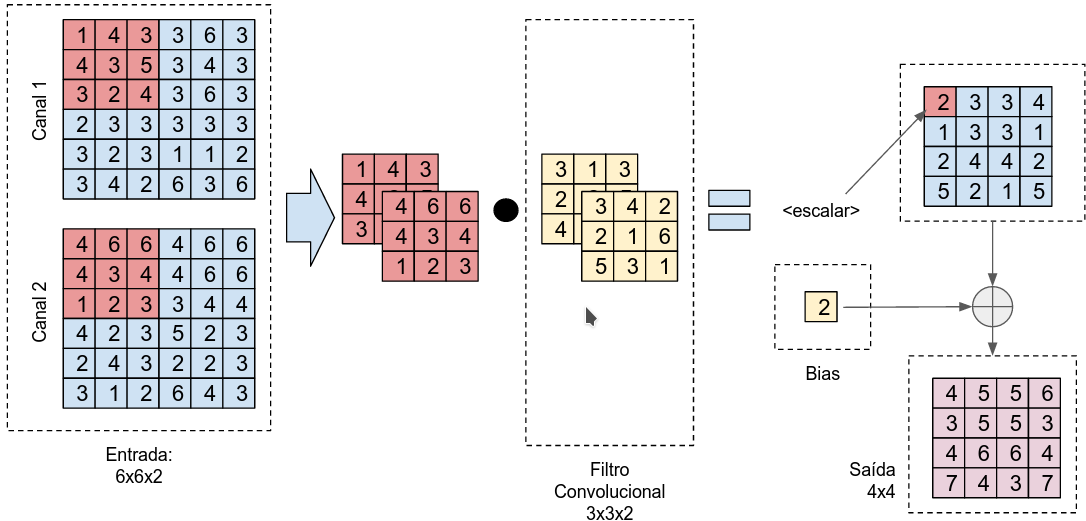
\includegraphics{ex_conv_2d.png}
	\caption{Exemplo de convolução 2D}
	\label{fig:ex_conv_2d}
	Exemplo da aplicação de uma única convolução sendo aplicada a uma imagem de
	entrada $6 \times 6 \times 2$. O tamanho da última dimensão do filtro e
	da entrada precisam ser iguais, no caso 2. As dimensões $3 \times 3$ do
	filtro foram escolhidas arbitrariamente. O símbolo do círculo na imagem
	representa um produto interno. A imagem de saída foi gerada deslocando
	a seleção de pixel a pixel até cobrir toda a
	imagem de entrada. Como as bordas não foram estendidas, a imagem
	resultante é menor que a de entrada (próprio autor).
\end{figure}

Camadas convolucionais também usam o conceito de bias. Para isso o tensor
resultante da convolução é somado a um escalar. Este escalar é treinável e
permite, entre outras coisas, que a rede neural gere valores não-nulos mesmo que
a entrada seja nula.

\subsection{Bordas} \label{ses:bordas}
Como já foi mencionado, a convolução é aplicado de forma idêntica a aplicação
de um filtro linear \cite{gonzalezwoods200708}, e assim como no caso dos
filtros lineares, existem algumas opções para tratamento de bordas dos dados.

Na figura \ref{fig:ex_conv_2d} o tamanho do tensor de saída foi reduzido
de 6 para 4. Neste caso a opção foi por não extender as bordas. Por
este motivo, o resultado tem que ser reduzida para impedir que o filtro
possua termos despareados.

Pode ser
desejável fazer a saída ter o mesmo tamanho da entrada. Para isso é necessário
estender as bordas da entrada, o que permitiria ao filtro ser deslocado por
toda a extensão entrada. Em camadas convolucionais observou-se apenas a
extensão com zeros. O software que foi adotado para a implementação deste
trabalho não suporta extensão que não seja com zeros, e não foi encontrado
\emph{paper} usando método diferente, como repetição.

A opção de extensão de borda é um hiperparâmetro.

\subsection{\emph{Stride}}
Ao se aplicar o filtro de convolução no tensor de entrada pode-se movê-lo de
posição a posição, até cobrir todos os locais válidos em cada direção, como
ilustrado na figura \ref{fig:ex_conv_2d}, ou pode-se desejar aplicar a cada
``$n_0$'' pixels em uma direção, ``$n_1$'' pixels em outra direção, e assim
por diante.  Esta opção é denominada \emph{stride}.

Quando uma camada convolucional possui como entrada um tensor de dimensões
$d1\times d2 \times ... \times dj \times C$, o stride é definido como sendo
um tensor unidimensional de tamanho j.
O stride $[1,2,1]$, por exemplo, indica que na primeira dimensão o
filtro será aplicado em todas as posições válidas, na segunda dimensão será
aplicado a cada 2 pixels e na terceira será aplicada novamente em todas as
posições válidas. Stride maior que 1 causa redução no tamanho do tensor de
saída.

Se um stride $2 \times 2$ fosse aplicado na convolução da figura
\ref{fig:ex_conv_2d} a imagem de saída seria $2 \times 2$.

\subsection{Profundidade do Filtro}
A figura \ref{fig:ex_conv_2d} mostrou um único filtro sendo aplicado ao
tensor de entrada. No entanto, é possível aplicar um número arbitrário
deles, sendo que cada filtro produz um tensor de saída.

Se o tensor de entrada possui dimensões $d0 \times d1 \times ... \times C$
e deseja-se aplicar sobre este
tensor $N$ convoluções é possível representar isso com um único tensor
com dimensões
$N \times d0 \times d1 \times ... \times C$. Cada um dos filtros vai gerar
um tensor de saída, em um total de $N$. O
número de filtros é denominado “profundidade do filtro”. Todas as saídas podem
ser representadas em um único tensor com uma dimensão adicional. Usa-se a última
dimensão do tensor de saída para este fim. O motivo para isso é que cada uma
dessas saídas efetivamente se torna um “canal” de saída desta rede neural. No
exemplo da figura \ref{fig:ex_conv_2d}, se fossem aplicados 3 filtros a saída
seria um tensor $4 \times 4 \times 3$. Para isso o tensor que define o filtro
convolucional passaria a ser um
filtro de profundidade 3 descrito por um tensor de dimensões
$3 \times 4 \times 4 \times 2$.

\subsection{Processamento em Lotes}
Existem alguns cuidados especiais que devem ser tomados durante o treinamento de
redes neurais. Tomando o caso do treinamento supervisionado como exemplo, o
otimizador ajusta os parâmetros treináveis da rede neural para tentar reduzir o
erro. Para verificar se a alteração teve sucesso, a rede neural é
alimentada com
dados rotulados, e o valor de saída da rede neural é comparado com os dados
esperados. É conveniente fornecer vários exemplos rotulados, não apenas um, e
usar a média do erro para alimentar o otimizador. A ideia é que o valor passado
seja o mais representativo possível.

O número de imagens fornecidas é denominado ``tamanho do lote''. Se uma rede
neural trabalha com dados de dimensões $d0 \times d1 \times ... \times C$
podem-se agrupar “B” exemplos em
um único tensor, com dimensões $B \times d0 \times d1 \times ... \times C$.
As camadas convolucionais tratam cada
uma das imagens separadamente, conforme já foi descrito, e emite na sua saída um
único tensor que também usa uma dimensão adicional para agrupar as diferentes
imagens.

O valor de B não é um hiperparâmetro, mas sim um parâmetro de treinamento.

\subsection{Pooling}
Após a aplicação de uma camada convolucional pode-se aplicar uma camada de
\emph{pooling}, que é uma forma de subamostragem. A figura
\ref{fig:ex_maxpool} ilustra uma operação de maxpool, que é um tipo de
pooling.

\begin{figure}[!htb]
	\centering
	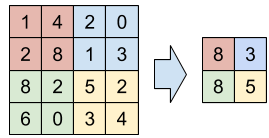
\includegraphics{ex_maxpool.png}
	\caption{Exemplo de \emph{maxpool} $2 \times 2$}
	\label{fig:ex_maxpool}
	Ilustração de uma operação maxpool $2 \times 2$ aplicado usando stride
	$2 \times 2$. O filtro move de dois em dois pixels e possui
	tamanho 2 em cada dimensão (próprio autor).
\end{figure}

Esta operação possui como parâmetros o tamanho do filtro, o stride e a opção de
borda. A operação a ser aplicada no filtro pode ser $max$ ou $avg$ (média),
que definem respectivamente os filtros \emph{maxpool} e \emph{avgpool}.

Como as operações de pooling são normalmente feitas com stride maior que 1 elas
acabam reduzindo consideravelmente o tamanho do tensor de saída. No caso de um
maxpool $2 \times 2$, por exemplo, o tensor resultante vai ter 25\% do
número de valores do tensor de entrada.

Uma camada convolucional com pooling pode ser contada como uma única camada ou
como duas, dependendo do caso. Em algumas arquiteturas mais complexas, como em
\cite{szegedy2015going}, onde define-se camadas do tipo \emph{inception},
pode não ser possível associar uma operação de \emph{pooling} a uma única
convolução, requerendo contagem separada.

\subsection{ReLu}
Assim como em redes neurais totalmente conectadas, pode-se aplicar uma função
de ativação para tornar a camada não-linear. As funções tangente
hiperbólica, sigmóide ou outras tipicamente usadas em redes neurais
não-convolucionais podem ser aplicadas. No entanto a função
\sigla{ReLu}{\emph{Rectified linear unit}, unidade linear retificada}, ou
linear retificada, resulta em treinamento substancialmente mais rápido enquanto
mantém a capacidade de generalização da rede neural treinada. A função
ReLu é definida por:


\begin{equation}
	ReLu(x) = max(0,x)
\end{equation}

Quando uma camada de uma rede neural inclui apenas elementos lineares,
ela é dita linear. O operador de convolução em sí é linear, então
isso vai ocorrer quando a camanda não inclui uma função de ativação, como
a ReLu e não possui outros elementos não-lineares, como \emph{maxpool},
caso o pooling esteja sendo considerado como parte da camada convolucional.

\subsection{Últimas Camadas}
Após as camadas convolucionais terem sido aplicadas é necessário usar um
classificador, mecanismo de regressão ou outro sistema que gere o tipo de saída
desejada para a rede neural. Uma das possíveis formas de realizar esta função é
usar uma ou duas camadas totalmente conectadas, como ilustrado na figura
\ref{fig:ex_cnn}. No exemplo a função de ativação da penúltima camada é
ReLu e a última camada é linear.

\subsection{Rede Neural Convolucional Completa}
Para alguns casos simples, pode-se construir uma rede neural convolucional
conectando-se uma camada convolucional a uma maxpool e uma ReLu. Este conjunto
pode ser repetido algumas vezes até que o número de saídas da camada
convolucional seja baixo o suficiente para que seja passado por duas camadas
totalmente conectadas. Se houver interesse em não reduzir o tamanho total do
tensor pode-se omitir a camada \emph{maxpool}. Um exemplo dessa topologia é a
figura \ref{fig:ex_cnn}.

A primeira camada da rede neural vai ter filtros que serão sensíveis a
características simples da entrada, que no caso de imagens seriam, por exemplo,
gradientes e trechos de linhas. Em
cada camada seguinte estas características são recombinadas com as detectadas
nas regiões vizinhas, formando conceitos progressivamente mais sofisticados a
respeito da imagem.

A topologia da rede neural e o conjunto de todos os hiperparâmetros definem o
número de parâmetros treináveis que a rede neural vai possuir e quantas
operações são necessárias para aplicar a rede neural em um (ou um lote de)
amostras. Uma rede neural mais larga, com um maior número de filtros por
camadas, possui a capacidade de aprender mais \emph{features}. Redes neurais
mais profundas possuem capacidade de abstração maior, sendo capazes de inferir
a partir dos dados de entrada conceitos mais complexos.

\begin{figure}[!htb]
	\centering
	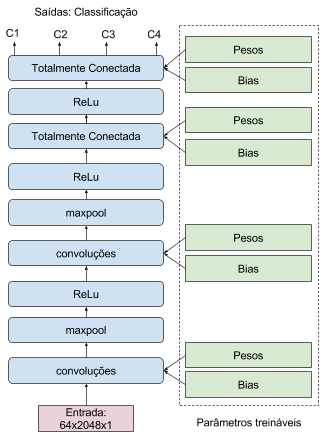
\includegraphics{ex_cnn.png}
	\caption{Exemplo de rede neural convolucional completa}
	\label{fig:ex_cnn}
	Esta rede neural possui nove camadas para
	classificação de séries temporais em uma de 4 classes. Destacam-se os
	parâmetros treináveis (próprio autor).
\end{figure}

\section{Uso em Processamento de Imagens}
O uso de redes neurais convolucionais é uma alternativa a diversos métodos já
existentes de detecção e reconhecimento de objetos em imagens. Aqui serão
mostradas algumas das alternativas usuais, para que sejam contrastadas
com a classificação baseada em redes neurais convolucionais.

\subsection{Redes Neurais Não-Convolucionais}
Quando uma imagem vai ser processada por uma rede não-convolucional ela precisa
ser convertida para a forma plana, em um vetor com dimensões
$H \cdot W \cdot C \times 1$.

O uso de camadas totalmente conectadas é proibitivo para classificação de
imagens desta maneira. Se uma rede neural for usada para processar imagens de 1
megapixel, ou $720 \times 1280$, e a primeira camada possuir um
número de neurônios igual
ao número de neurônios da camada de entrada, a matriz de pesos teria
$(720 \cdot 1280 \cdot 3)^2 \approx 7.6 \cdot 10^{12}$ parâmetros. Se for
representado por números ponto-flutuante de 32 bits isso ocuparia mais de
30 TiB. O mesmo processo em uma imagem 480px por 640px geraria quase 850
bilhões de parâmetros só na matriz de pesos.

Outras topologias mais esparsas podem ser construídas, mas este tipo de rede
neural possui outros problemas que as tornam inviáveis para processamento direto
de imagens. Um exemplo é o fato delas não serem invariantes ao deslocamento. Se
a rede neural aprende a reconhecer um \emph{feature} em um local da
imagem, não vai
conseguir reaproveitar essa capacidade em outras posições. Portanto teria que
aprender a mesma \emph{feature} em cada possível posição onde ela possa
aparecer, e fazer isso para todas as \emph{features}.

Como a primeira operação feita foi converter a imagem para um formato “plano”, a
geometria da imagem foi destruída. Não é mais possível determinar quando dois
pixels estão próximos, e essa é uma informação muito importante sobre a imagem.

\subsection{Uso de descritores}
Uma das abordagens possíveis para reconhecimento e detecção de imagens é o uso
de descritores. Esta foi a abordagem dominante até pouco tempo atrás.

Os descritores são operações que tomam uma imagem como entrada e resumem as sua
características em um set menor de informações. Exemplos de descritores muito
usados são
\sigla{LBP}{\emph{Local binary patterns}, padrões binários locais}
	\cite{wang1990texture},
\sigla{ORB}{\emph{Oriented FAST and rotated BRIEF}} \cite{rublee2011orb},
\sigla{HOG}{\emph{Histogram of oriented gradients}, histograma de gradientes
	orientados} \cite{dalal2005histograms},
Haar-Wavelets \cite{nabout2008object},
filtros de Gabor \cite{riaz2012invariant}.
O treinamento é realizado sobre
as features extraídas pelo descritor escolhido usando um classificador como
redes neurais ou \sigla{SVM}{\emph{Support vector machine}}.

Para usar esta abordagem um descritor precisa ser escolhido e configurado,
muitas vezes manualmente. O desempenho do sistema como um todo vai depender
dessas escolhas. Se a operação de detecção depender de conceitos complexos,
envolvendo correlação entre múltiplas características, o descritor e o
classificador precisam ser escolhidos especificamente para isso.

\subsection{Redes Neurais Convolucionais em Imagens}
As redes neurais convolucionais operam diretamente nos pixels da imagem, não
sendo necessário escolher um descritor, e não possuem os problemas que as
redes não-convolucionais possuem. As camadas convolucionais se comportam como
descritores, porém os parâmetros são aprendidos como parte do processo de
treinamento, portanto são otimizados para responderem precisamente para os
exmeplos que forem fornecidos. Apenas alguns hiperparâmetros, como tamanho
da convolução, número de filtros e de camadas precisam ser escolhidos mediante
decisões de meta de precisão e recall, tempo para classificação e complexidade
dos conceitos a serem aprendidos.

As redes neurais convolucionais resolvem todos esses problemas simultaneamente.
O primeiro ponto é a preservação da geometria da imagem. Se uma imagem de 50
pixels de altura por 100 pixels de largura contendo 3 canais de cor for usado na
entrada de uma rede neural convolucional, ela precisa ser representada por um
tensor apropriado, como $32 \times 50 \times 100 \times 3$. Este tensor
permite alimentar a rede neural com um lote de 32 imagens.

Para aplicar uma camada convolucional à imagem de entrada escolhe-se o tamanho
da convolução, o número de filtros e o modo de operação nas bordas. A figura
\ref{fig:ex_cnn_img} ilustra um filtro 33 sendo aplicado a uma imagem
\sigla{RGB}{\emph{Red, green, blue}, vermelho, verde, vermelho}.

\begin{figure}[!htb]
	\centering
	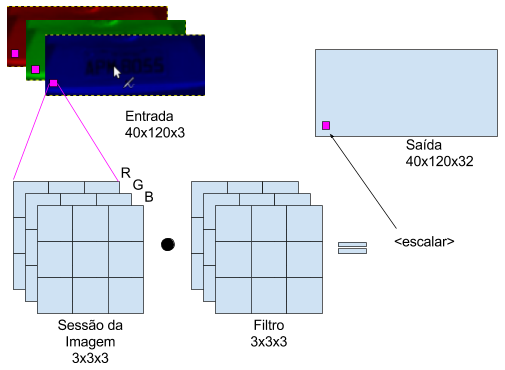
\includegraphics{ex_cnn_img.png}
	\caption{Convolução sendo aplicada em uma imagem RGB}
	\label{fig:ex_cnn_img}
	Como a imagem possui 3 canais o filtro será $3 \times 3 \times 3$.
	Uma partição da imagem original com o mesmo tamanho do filtro,
	$3 \times 3 \times 3$ é extraído da imagem, e um
	produto interno é realizado entre os dois, resultando em um escalar. Este
	escalar é armazenado no tensor de saída nas coordenadas corretas. A
	ilustração só mostra uma imagem de entrada e só um filtro e, portanto, uma
	imagem de saída (próprio autor).
\end{figure}

Para que o filtro tenha profundidade 64, por exemplo, o tensor que define o
filtro será $64 \times 3 \times 3 \times 3$ e o tensor resultante da
convolução será $32 \times 40 \times 120 \times 64$,
considerando que seja usado preenchimento nas bordas.

Para finalizar a camada convolucional adiciona-se um bias. Para isso usa-se um
escalar para cada uma das 64 imagens resultantes. O tensor que define os bias é
um tensor unidimensional com tamanho 64.

Camadas maxpool e ReLu podem ser adicionadas para reduzir as dimensões da imagem
ou aumentar a sua não-linearidade. A figura \ref{fig:ex_full_cnn_img}
ilustra o uso das três camadas em sequência.

\begin{figure}[!htb]
	\centering
	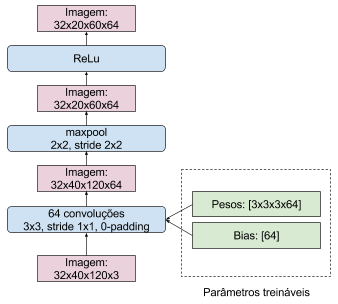
\includegraphics{ex_full_cnn_img.png}
	\caption{Exemplo de rede neural convolucional completa aplicada à uma imagem
	RGB}
	\label{fig:ex_full_cnn_img}
	Exemplo de uma sequência de operações feitas usando uma rede neural
	convolucional incluindo 64 convoluções $3 \times 3$, maxpool e ReLu
	aplicadas em uma
	lote de 32 imagens $40 \times 120 \times 3$. Os parâmetros treináveis
	estão destacados (próprio autor).
\end{figure}

A imagem é tratada por camadas sucessivas de convolução, maxpool e ReLu até que
o tamanho total do tensor seja pequeno o suficiente para poder ser processado
por duas camadas totalmente conectadas. 

\subsection{Uso de Cores}
Em alguns sistemas de visão computacional são usadas imagens em
tons de cinza. No caso de redes convolucionais o mais comum é usar
imagens coloridas.

O primeiro motivo para isso é que as imagens e vídeos são normalmente
captadas com cores, então o processo de detecção teria que incluir uma operação
de conversão para escala de cinza. 

Pode-se demonstrar todos os métodos de conversão lineares de RGB para escala de
cinzas, como:

\begin{equation} \label{eq:rgb2gray}
	G=0.299R + 0,587G + 0.114B
\end{equation}

Podem ser representados como uma convolução $1 \times 1$. Visto que as
convoluções são implementadas de forma bastante eficientes nas bibliotecas
de redes neurais convolucionais, algumas vezes até usando aceleração por
hardware, então não necessariamente haverá economia durante a execução
durante a execução da rede neural, pois, no pior caso, ela mesma pode fazer
essa conversão de forma eficiente, sendo que os coeficientes associados
à cada canal, que no exemplo da equação \ref{eq:rgb2gray} são fixos, podem
treinados pelo otimizador, potencialmente obtendo uma conversão mais apropriada
para a rede neural.

Outro ponto é que os sistemas que representam o atual
estado-da-arte para reconhecimento de imagem, como \cite{szegedy2015going}
\cite{hasanpour2016lets}, usam cores, portanto nos casos onde
existe \emph{budget} computacional, e particularmente quando é possível usar
vários filtros convolucionais na primeira camada, a informação da cor pode
ser vantajosa para para minimizar os erros da rede neural.

\subsection{Reconhecimento de Objetos}
Existem várias maneiras de se usar redes neurais para reconhecer objetos. Duas
das opções envolvem configurar a neural como classificador e como sistema de
regressão.

Para usar a rede como classificador pode-se incluir na última camada da rede
neural um sistema softmax, também conhecido como exponencial normalizada. Isso
permite que a rede neural seja treinada e, após o treinamento, estime a
probabilidade da sua entrada pertencer a cada uma de N classes. A rede neural é
implementada usando $N$ saídas, de forma que cada saída é treinada para
representar a probabilidade da entrada ser classificada em em uma das classes.
Uma saída \emph{softmax} realiza uma normalização das saídas da rede neural,
usando a equação:

\begin{equation}
	softmax[i] = \frac
		{exp\left( \widehat{out}[i] \right)}
		{\sum_j exp\left( \widehat{out}[j] \right)}
\end{equation}

Para identificar a presença ou não do objeto que está sendo procurado, duas
classes seriam definidas: ``presente'' e ``não-presente'', resultando em uma rede
neural como mostrada na figura \ref{fig:ex_classif_logist}.

\begin{figure}[!htb]
	\centering
	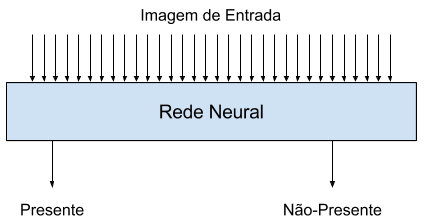
\includegraphics{ex_classif_logist.png}
	\caption{Exemplo de Classificador Logístico}
	\label{fig:ex_classif_logist}
	Este exemplo de rede neural possui uma imagem como entrada e possui duas
	saídas, uma informando a probabilidade da imagem conter o objeto, outra
	indicando a probabilidade de não conter (próprio autor).
\end{figure}

Este modelo pode ser treinado usando modo supervisionado, onde imagens
pré-classificadas são fornecidas. A função de perda a ser minimizada pelo
otimizador é a função \emph{cross entropy}:

\begin{equation}
	\widehat{H} = - \sum_i \widehat{y_i} log(y_i)
\end{equation}

Onde $y_i$ é o valor da probabilidade manualmente
marcadas de uma imagem pertencer à classe $i$ (no caso, a probabilidade de ser
uma imagem que contém o objeto e a probabilidade não conter) e $\widehat{y_i}$
é o valor estimado pela rede neural. $H$ é o valor estimado de
\emph{cross entropy}.

Quando têm-se o objeto desejado centrado na imagem, ou o objeto não consta
em lugar nenhum da imagem usa-se os valores $0$ e $1$ para rotular os exemplos.
Os casos onde o objeto está visível apenas parcialmente deve ser considerado
cuidadosamente, produzindo valores intermediários nos rótulos, para evitar que
duas imagens parecidas gerem valores muito diferentes na saída da rede neural.

As redes neurais também podem ser usadas para fazer regressão, ou seja, modelar
uma função. A forma mais óbvia de implementação é a regressão L2. Neste tipo de
função o otimizador vai minimizar o erro quadrático:

\begin{equation}
	E=sum \left( \left( y - \widehat{y} \right)^2 \right)
\end{equation}

Sendo que $sum$ é uma função que representa a soma de todos os valores do
tensor que recebe como parâmetro.
A rede neural pode ser usada para modelar a função $P$, definida por:

\begin{equation}
	y = P(img) = \begin{cases}
		1 \text{, se img contém o objeto procurado} \\
		t(img) \text{, se objeto está parcialmente visível} \\
		0 \text{, se img não contém}
	\end{cases}
\end{equation}

Detectores podem encontrar o objeto que estão procurando parcialmente presentes 
no seu campo de visão, e esta função precisa tratar desta possibilidade. No
caso a condição de transição, representada por $t(img)$, não está sendo
aqui definida, pois implementação deve escolher esta função cuidadosamente
para integração com o \emph{software} que vem depois da rede neural.
Uma coisa que não pode ocorrer é descontinuidade entre duas imagens próximas,
especialmente no caso de translação, pois o otimizador teria que encontrar
pesos que modelassem a descontinuidade, e mesmo uma pequena imprecisão nestes
pesos vai gerar um erro muito grande.

\subsection{Localização de Objetos} \label{sec:localiz_objetos}
Até agora foi mostrado como usar redes neurais convolucionais para detectar um
objeto em uma imagem. Isso envolve apenas determinar se uma imagem possui ou não
o objeto de interesse. Localização, ao contrário, requer a determinação das
coordenadas do objeto.

Um sistema de localização pode ser construído a partir de um sistema de
detecção. A abordagem mais simples para isso envolve construir um sistema capaz
de detectar o objeto de interesse e aplicar este
detector à imagem várias vezes a imagem usando ``janelas deslizantes''.
Se o detector for construído para produzir “1” quando detectar o objeto e
“0” então os pontos de máxima são candidatos a centros dos objetos.

Como cada pixel da imagem é candidato a centro do objeto que está sendo
localizado, deve-se aplicar o filtro uma vêz para cada pixel. Se não houver
extensão de bordas, o filtro não pode ser aplicado em parte dos pixels.
